\documentclass[a4paper]{jpconf}
%\bibliographystyle{iopart-num}
%\usepackage{citesort}
\usepackage{graphicx}
\begin{document}
\title{Ideal $\tau$ tagging with TMVA multivariate data-analysis toolkit}

\author{A Heikkinen, P Kaitaniemi, V Karim\"{a}ki,
M~J Kortelainen, T~Lamp\'{e}n, S Lehti, T Lind\'{e}n and L Wendland} 

\address{Helsinki Institute of Physics, P.O. Box 64, FIN-00014 University of Helsinki, Finland}

\ead{aatos.heikkinen@cern.ch}


\begin{abstract}
We report our experience on using ROOT package TMVA for
multivariate data analysis, for a problem of $\tau$ tagging in the
framework of heavy charged MSSM Higgs boson searches at the LHC.
With a generator level analysis,
we investigate how in the ideal case $\tau$ tagging could be performed and
hadronic $\tau$ decays separated from the
hadronic jets of QCD multi-jet background present in LHC experiments.
A successful separation of the Higgs signal from the background
requires a rejection factor of $10^5$ or better against the QCD background.
The $\tau$ tagging efficiency and background rejection are studied with various MVA classifiers.
\end{abstract}


\section{Introduction}
\cite{abla}


\section{A new physics list}

%We have implemented a new physics list called {\sf QGSP\_\-INCL\_ABLA} with

 
%\begin{figure}[h]
% \begin{minipage}{7.0cm}
%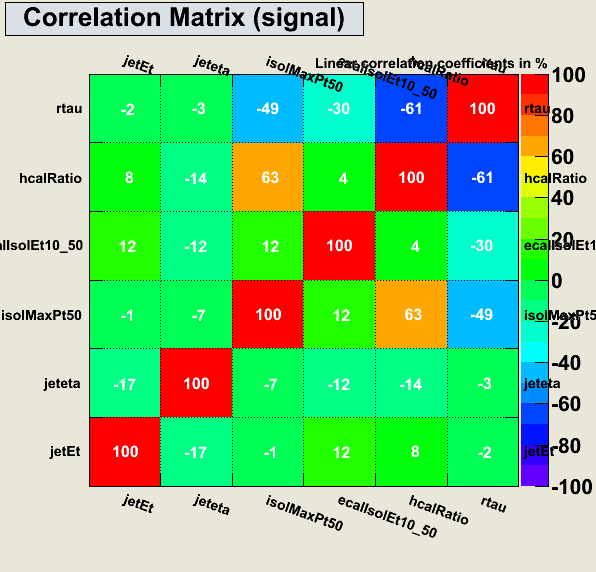
\includegraphics[width=1.0\textwidth]{images/ahCorrelationMatrixS.png}
%\end{minipage}
% \hfill
%\begin{minipage}{7.0cm}
%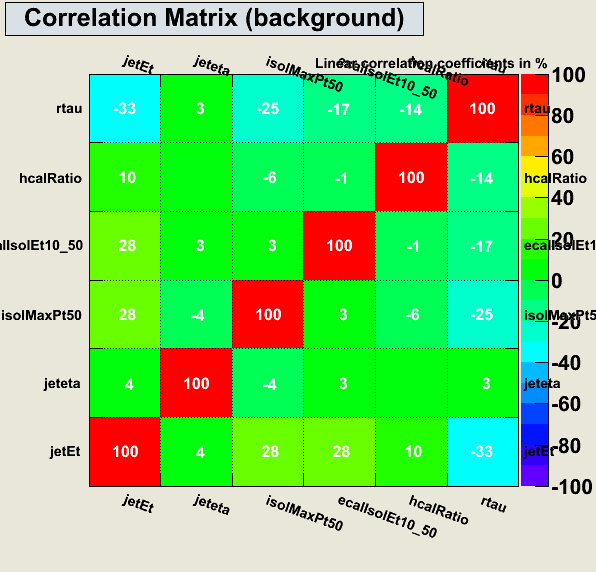
\includegraphics[width=1.0\textwidth]{images/ahCorrelationMatrixB.png}
%\end{minipage}
%\begin{minipage}{3.0cm}
%\caption{Right: Variable correlation matrix for signal Right: Variable correlation matrix for background}
%\end{minipage}
%\label{fig:ahCorrelationMatrix}
%\end{figure}


\subsection{Event evaluation}
Pseudo-pseudocode of the event evaluation
\scriptsize
\begin{verbatim}
Infer cut orientation for each classifier from TMVA classifier output distributions

Separate classifiers to cuts and non-cuts classifiers

Create TTreeFormula objects corresponding to the TMVA preselection cuts

Initialize TMVA Reader

Initialize temporary TTree for non-cuts classifier output values

Book classifiers on reader and set branches for classifier output values

For each entry in signal and background testing TTree
  If entry doesn't pass preselection cuts
    Continue to next entry

  Get variable values from TTreeFormula

  For each non-cuts classifier
    Compute classifier output from the entry

  If current entry belongs to a different event as the previous entry
    Fill the non-cuts classifier outputs from the previous event to the temporary TTree
    Store classifier outputs from current event to the buffer
  Else
    For each non-cuts classifier
      Take min/max (depending on the cut orientation) of the buffered output value and the value from this entry,
      and store it to the buffer

  For each cuts classifier
    For each ROC bin
      If entry passes the cuts corresponding the signal efficiency value of the ROC bin
        If this event has not yet been marked as added for this ROC bin
          Add event as passed for this ROC bin

Fill the non-cuts classifier outputs from the last event to the temporary TTree

Calculate event/jet preselection efficiencies and print them

For each entry in the temporary TTree
  For each non-cuts classifier
    Fill classifier output histogram
    Fill classifier efficiency histogram

For each non-cuts classifier
  Normalize efficiency histogram
  For each ROC bin
    Get the signal efficiency value of the ROC bin
    Find the classifier output cut value corresponding to the signal efficiency
    Obtain background efficiency by imposing the the cut on background distribution
    Add background efficiency value to the ROC bin

For each cuts classifier
  Normalize efficiency histogram
  For each ROC bin
    Get the signal and background efficiencies for that bin
    Add the point to the ROC curve 

Print efficiency tables
\end{verbatim}
\normalsize

\subsection{SVM}

\begin{itemize}
\item Training 4000 signal jets, 32000 background jets
\item Optimization was a 2D scan in the $\sigma, C$ parameter space
  \begin{itemize}
  \item A grid was set up in this space
  \item The training and evaluation for each point was run in parallel in a Linux cluster
  \end{itemize}
\item Results
  \begin{itemize}
  \item Background 1
    \begin{itemize}
    \item $10^{-5}$ bkg eff: $5.68\pm 0.12\;\%$
    \item $10^{-6}$ bkg eff: $1.66\pm 0.06\;\%$
    \end{itemize}
  \item Background 2
    \begin{itemize}
    \item $10^{-5}$ bkg eff: $5.49\pm 0.12\;\%$
    \item $10^{-6}$ bkg eff: $1.80\pm 0.07\;\%$
    \end{itemize}
  \item Figures \ref{fig:mkSvmGauss2} and \ref{fig:mkSvmParallels}
  \end{itemize}
\end{itemize}

 
\begin{figure}[h]
 \begin{minipage}{7.0cm}
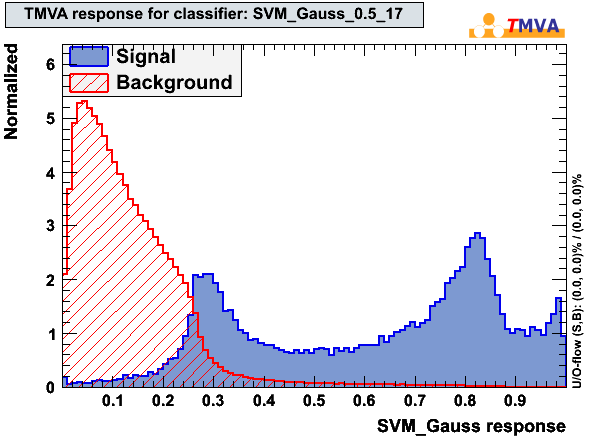
\includegraphics[width=1.0\textwidth]{images/mk_svm_gauss2.png}
\end{minipage}
 \hfill
\begin{minipage}{7.0cm}
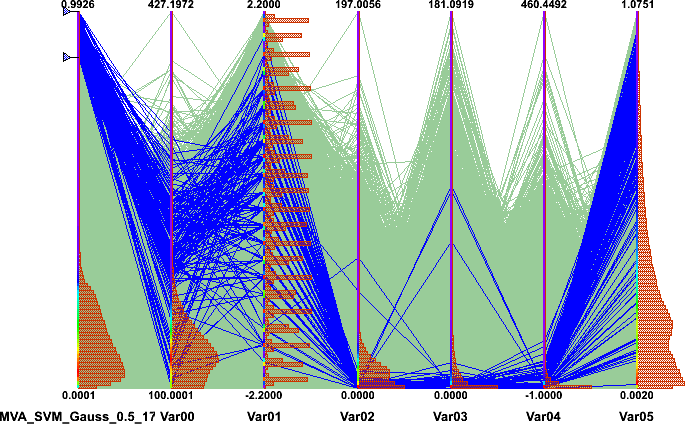
\includegraphics[width=1.0\textwidth]{images/svm_parallels2.png}
\end{minipage}
\begin{minipage}{3.0cm}
\caption{AH:::}
\end{minipage}
\label{fig:ahCorrelationMatrix}
\end{figure}


\begin{figure}[h]
\begin{center}
%\includegraphics[width=21pc]{poster/images/.png}\hspace{2pc}%
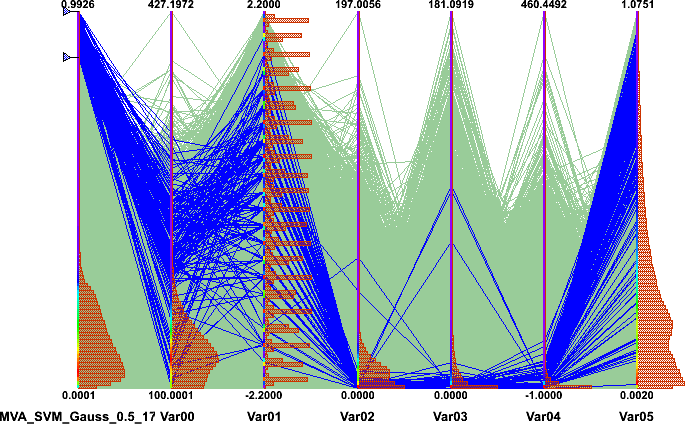
\includegraphics[width=1.0\textwidth]{images/svm_parallels2.png}
%\begin{minipage}[b]{14pc}
\caption{\label{label}AH:::}
%\end{minipage}
\end{center}
\end{figure}


%Perusasetus, ei VarTransformia
%Fisher H:!V:!Normalise:CreateMVAPdfs:Fisher:NbinsMVAPdf=50:NsmoothMVAPdf=1
%HMatrix H:!V:CreateMVAPdfs
%--------------------
%       data1           data2
%Fisher  0.0352(009)     0.0352(009)
%HMatrix 0.0106(005)     0.0104(005)

\begin{figure}[h]
\begin{center}
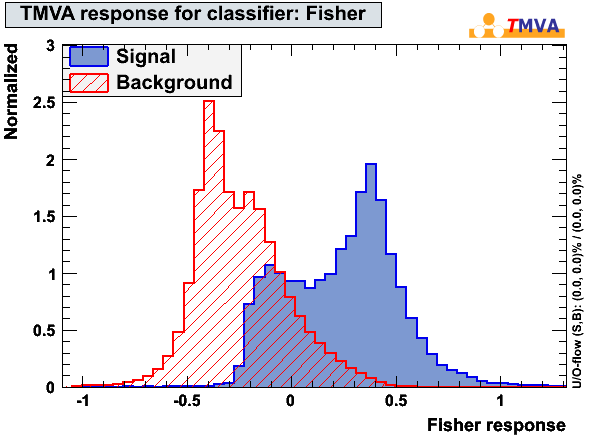
\includegraphics[width=1.0\textwidth]{images/mva_Fisher.png}
\caption{\label{label}AH:::}
\end{center}
\end{figure}

\begin{figure}[h]
\begin{center}
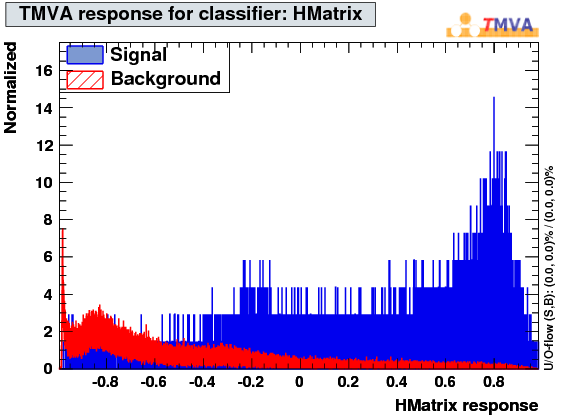
\includegraphics[width=1.0\textwidth]{images/mva_HMatrix.png}
\caption{\label{label}AH:::}
\end{center}
\end{figure}


\begin{figure}[h]
\begin{center}
%\includegraphics[scale=0.70]{poster/images/fragments.eps}

%\caption{Fragment production of the INCL and ABLA \cite{abla, abla1, abla2} models. 
%and new C++ implementation, respectively. Data is from Ref. \cite{gsifragments}.}
\label{fig:neutronAl}
\end{center}
\end{figure}


%\begin{figure}[h]
%\begin{minipage}{14pc}
%\begin{center}
%\includegraphics[width=30pc]{poster/images/lead.eps}
%\end{center}
%\caption{\label{label}Figure caption .}
%\end{minipage}\hspace{2pc}%
%\begin{minipage}{14pc}
%\includegraphics[width=14pc]{./poster/images/inclAblaDoc.eps}
%\caption{\label{label}Figure caption for second of two sided figures.}
%\end{minipage} 
%\end{figure}


% \ack %command \ack sets the acknowledgments heading as an unnumbered section.


%\appendix % The command \appendix" is used to signify the start of the appendixes.
%\section{AH:::}

%\begin{equation}
%time= money
%\end{equation}

%To obtain a simple heading of `Appendix' use the code \verb"\section*{Appendix}". 
%If it contains numbered equations, figures or tables the command \verb"\appendix" should
%precede it and \verb"\setcounter{section}{1}" must follow it. 



\begin{center}
\begin{table}[h]
\caption{\label{opt}Summary of {\sf QGSP\_\-INCL\_ABLA} physics list.}
%\footnotesize\rm
\centering
\begin{tabular}{@{}*{7}{l}}
\br
Option&Description\\
\mr
\verb"Al-"&Targets heavier than Aluminium.\\
\verb"150~MeV -"&Projectile energies from $\sim$ 150 MeV up to 2.5 GeV $\sim$ 3 GeV.\\
\br
\end{tabular}
\end{table}
\end{center}



\section*{References}

\begin{thebibliography}{9}

%\bibitem{incl} A. Boudard et al., \emph{Intranuclear cascade model for
%    a comprehensive description of spallation reaction data}, Phys.
%  Rev. C66 (2002) 044615
%\bibitem{g4} \emph{Geant4 collaboration website} \\ {\tt http://\-cern.ch/\-geant4}
%\bibitem{pk08bProceedings}
%A. Heikkinen, P. Kaitaniemi, and A. Boudard,
%{\em Implementation of INCL4 cascade and ABLA evaporation codes in Geant4},
%Journal of Physics: Conference Series 119 (2008) 032024, 
%{\sf [doi:10.1088/1742-6596/119/3/032024]}
\bibitem{abla} J. Benlliure et al., \emph{Calculated nuclide
    production yields in relativistic collisions of fissile nuclei},
  Nuc. Phys. A628 (1998) 458
\bibitem{abla1} J. J. Gaimard et al., \emph{},
  Nuc. Phys. A531 (1991) 709
\bibitem{abla2} A. R. Junghans et al., \emph{},
  Nuc. Phys. A629 (1998) 635
\bibitem{gsifragments} T. Enqvist et al. \emph{},
  Nucl. Phys. A686 (2001) 481
\bibitem{g4incl} \emph{Geant4 Physics Reference Manual: INCL~4.2 Cascade and ABLA~V3 Evaporation with Fission} 
%\\ {\tt http://geant4.web.cern.ch/\-geant4/\-UserDocumentation/\-UsersGuides/\-PhysicsReferenceManual/\-html/\-node185.html}

\bibitem{data} X.Ledoux et al., \emph{Spallation Neutron Production by
  0.8, 1.2, and 1.6 GeV Protons on Pb Targets} Phys. Rev. Lett. 82
  (1999)

%\item Strite S and Morkoc H 1992 {\it J. Vac. Sci. Technol.} B {\bf 10} 1237 
\end{thebibliography}


\end{document}



